\chapter{Prueba de concepto}
\label{pruebaconcepto}

En este capítulo se va a hablar de una pequeña prueba de concepto que consiste en un escenario \ac{SDN}-\ac{NFV} donde todas las \acp{API} y herramientas mencionadas en los capítulos \ref{herramientas} y \ref{desarrollo} trabajan conjuntamente en total sintonía.

Inicialmente, se habla sobre el contexto en el que se ha enmarcado la prueba de concepto, haciendo especial referencia al Proyecto H2020 Metro-Haul\cite{metrohaulbib}.

A continuación, se establece una arquitectura de desarrollo, en la que se define el papel de cada \ac{API} y herramienta, y como interactúan entre sí.

Por último, se realiza una explicación del funcionamiento de la prueba de concepto, así como una vista de los resultados finales.

\section{Contexto}
\label{sec:contexto}

Esta prueba de concepto está enmarcada dentro del proyecto europeo H2020 Metro-Haul\cite{metrohaulbib}. Su principal objetivo es el de diseñar arquitecturas de redes metro que sean accesibles para 5G, anticipándose a los posibles problemas futuros cuando 5G esté totalmente funcional en las redes de telecomunicación.

Estas nuevas arquitecturas aseguran que algunos parámetros de calidad de servicio, como la latencia o el \textit{jitter} sean lo más bajos posibles, así como una total integración de nuevas tecnologías referentes al campo de \ac{ICT}, como son \ac{SDN} y \ac{NFV}.

Para conseguir todos estos objetivos, Metro-Haul busca integrar diferentes herramientas para diseñar nuevas arquitecturas de red. Esta prueba de concepto se planteó como una demostración de como diferentes herramientas podían operar en sintonía para disminuir la latencia al establecer diferentes \textit{Service Chains}, anticipando la llegada del 5G.\cite{demoecocbib}

Dicha demostración tuvo éxito y se publicó en el congreso internacional \ac{ECOC}\cite{ecocbib} en Septiembre de 2018.

\section{Arquitectura}
\label{sec:arquitectura}

El principal objetivo de la prueba de concepto es el de integrar todas las \acp{API} y herramientas mencionadas anteriormente para conseguir satisfacer diferentes \textit{Service Chains} con restricciones de latencia y ancho de banda. Además, se busca demostrar como todas las herramientas \textit{open-source} que componen dicha prueba de concepto trabajan en sintonía para crear un escenario \ac{SDN}-\ac{NFV} heterogéneo.

Para conseguir los objetivos mencionados anteriormente, se ha diseñado una arquitectura específica para poder llevar a cabo la prueba de concepto, donde cada uno de los elementos realiza una tarea en concreto.

\begin{figure}[!ht]
	\centering
	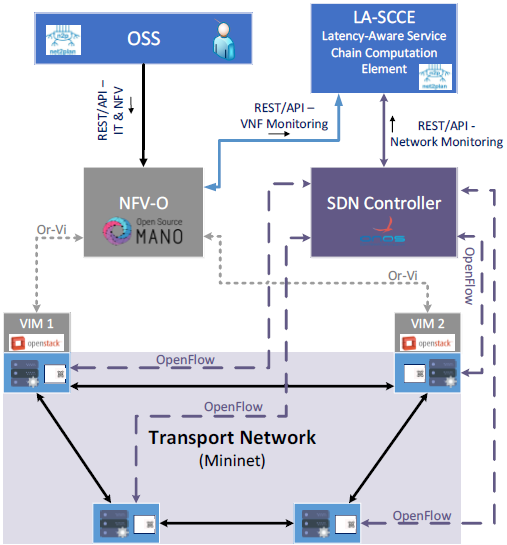
\includegraphics[width=0.7\linewidth]{imagenes/esquema_demo}
	\caption{Arquitectura de la Prueba de Concepto. Fuente:\cite{demoecocbib}}
	\label{fig:esquemademo}
\end{figure}

En la figura \ref{fig:esquemademo} se puede observar un esquema de la arquitectura, en el que se incluyen todos los elementos que la componen, y hace más fácil de entender como interactúan entre sí los componentes.

A continuación vemos una explicación de cada uno de los elementos que componen la prueba de concepto y que componente lleva a cabo esa acción:

\begin{itemize}
	\item \textbf{\ac{OSS}:} representa el papel de un operador que despliega un servicio gracias a una aplicación. El operador es emulado mediante la \ac{GUI} de Net2Plan, más concretamente por su plugin de \textit{NFV Management} (ver \ref{sec:nfvplugin}).
	
	\item \textbf{\ac{NFV-O}:} representa el papel de una aplicación que se encarga de gestionar la infraestructura de virtualización necesaria para instanciar diferentes máquinas virtuales. \ac{OSM} (ver \ref{sec:osm}) es el encargado de dicha función.
	
	\item \textbf{\acp{VIM}:} son los encargados de instanciar y alojar las diferentes máquinas virtuales pertenecientes a los VNF. OpenStack (ver \ref{sec:openstack}) es quien realiza este papel.
	
	\item \textbf{Red de Transporte:} la red de transporte es emulada mediante Mininet (ver \ref{sec:mininet}) para establecer flujos de paquetes entre las diferentes \acp{VNF} de una \textit{Service Chain}. La red se define mediante un script en Python (ver anexo \ref{sec:scriptmininet}).
	
	\item \textbf{Controlador \ac{SDN}:} la red de transporte es controlada por una instancia de \ac{ONOS} (ver \ref{sec:onos}) mediante el envio de paquetes Openflow (ver \ref{subsec:openflow}) a los diferentes switches de la red.
	
	\item \textbf{\ac{LA-SCCE}:} Se encarga de decidir el camino a seguir para atravesar una secuencia de \acp{VNF} que cumpla con los requisitos de latencia máxima. Este papel lo representa un algoritmo programado en Net2Plan para resolver de forma conjunta tanto el camino como el emplazamiento de las \acp{VNF} óptimos.
\end{itemize}


\section{Funcionamiento}
\label{sec:funcprueba}

Para llevar a cabo la prueba de concepto, la arquitectura explicada en la sección anterior se ha traducido en un \textit{testbed} para poder llevarla a cabo, como se puede apreciar en la figura \ref{fig:poctestbed}.

\begin{figure}[!ht]
	\centering
	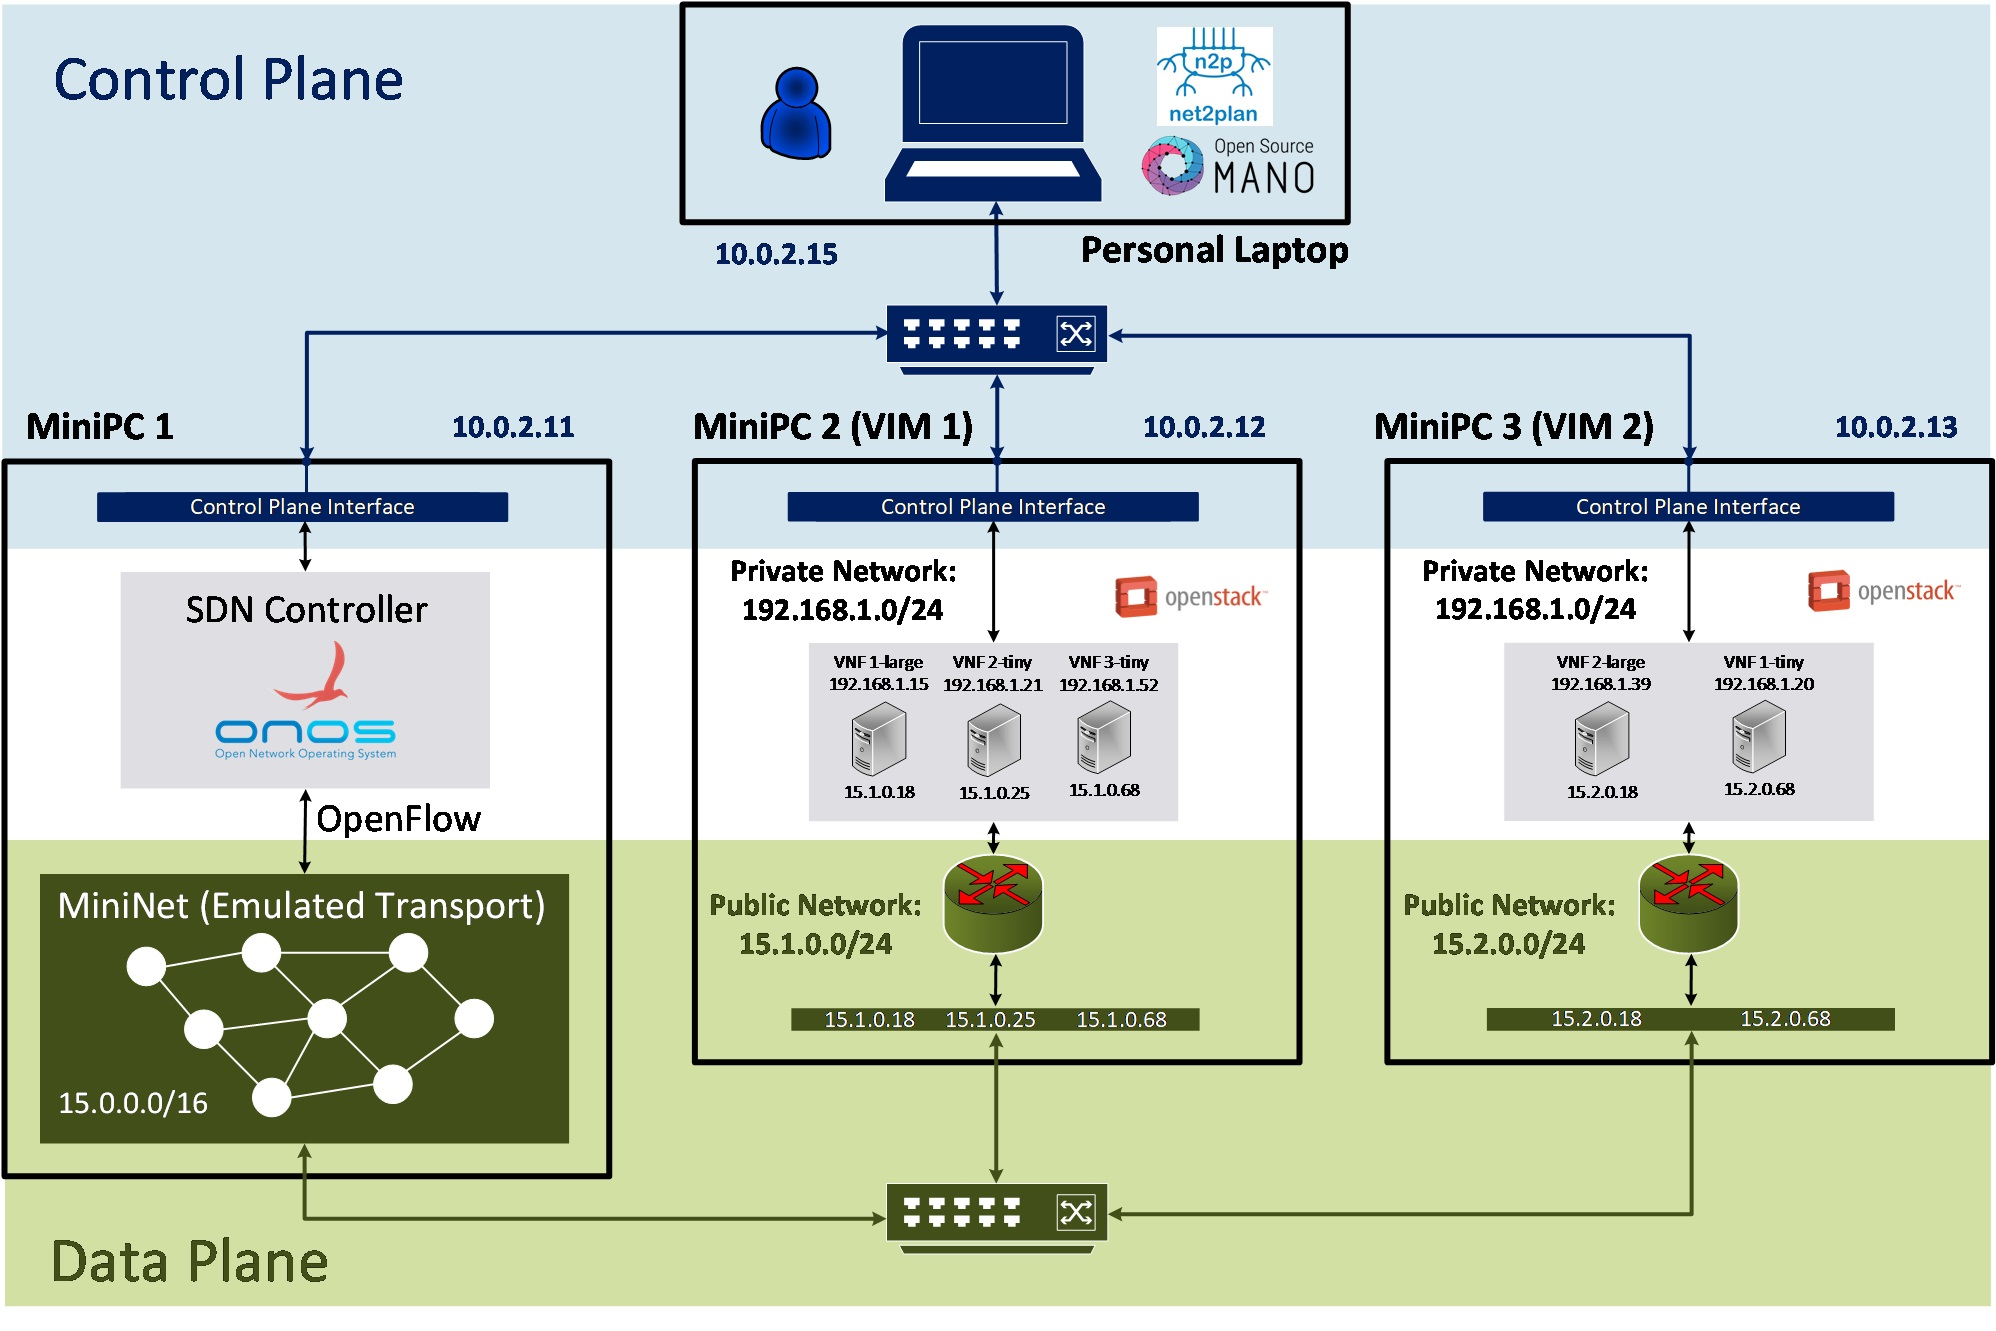
\includegraphics[width=0.9\linewidth]{imagenes/PoC_testbed}
	\caption{\textit{Testbed} para la Prueba de Concepto. Fuente:\cite{demoecocbib}}
	\label{fig:poctestbed}
\end{figure}

El \textit{testbed} considerado se compone de cuatro \acp{PC} y dos \textit{switches}, uno para el plano de control y otro para el plano de datos:

\begin{itemize}
	\item \textbf{Mini\ac{PC}1:} Este \ac{PC} se encarga de alojar una instancia del controlador \ac{SDN} \ac{ONOS} y de emular la red de transporte gracias a Mininet.
	
	\item \textbf{Mini\ac{PC}2:} En este \ac{PC} se encuentra corriendo una instancia de OpenStack, que actúa como \ac{VIM} 1.
	
	\item \textbf{Mini\ac{PC}3:} En este \ac{PC} se encuentra corriendo una instancia de OpenStack, que actúa como \ac{VIM} 2.
	
	\item \textbf{\textit{Personal Laptop}:} Este dispositivo actúa como entidad central del \textit{testbed}. En él se encuentra corriendo una instancia de \ac{OSM} y el plugin \textit{NFV Management} de Net2Plan.
\end{itemize}


Una vez explicado el \textit{testbed}, se explican los diferentes pasos que se realizan para llevar a cabo la prueba de concepto y que \acp{API} intervienen en cada uno de ellos:

\begin{itemize}
	
	\item \textbf{Paso 1.} Una vez que \ac{ONOS}, \ac{OSM} y los \acp{VIM} estan listos y corriendo, se arranca el plugin de Net2Plan para comenzar con la demostración.
	
	\begin{figure}[!ht]
		\centering
		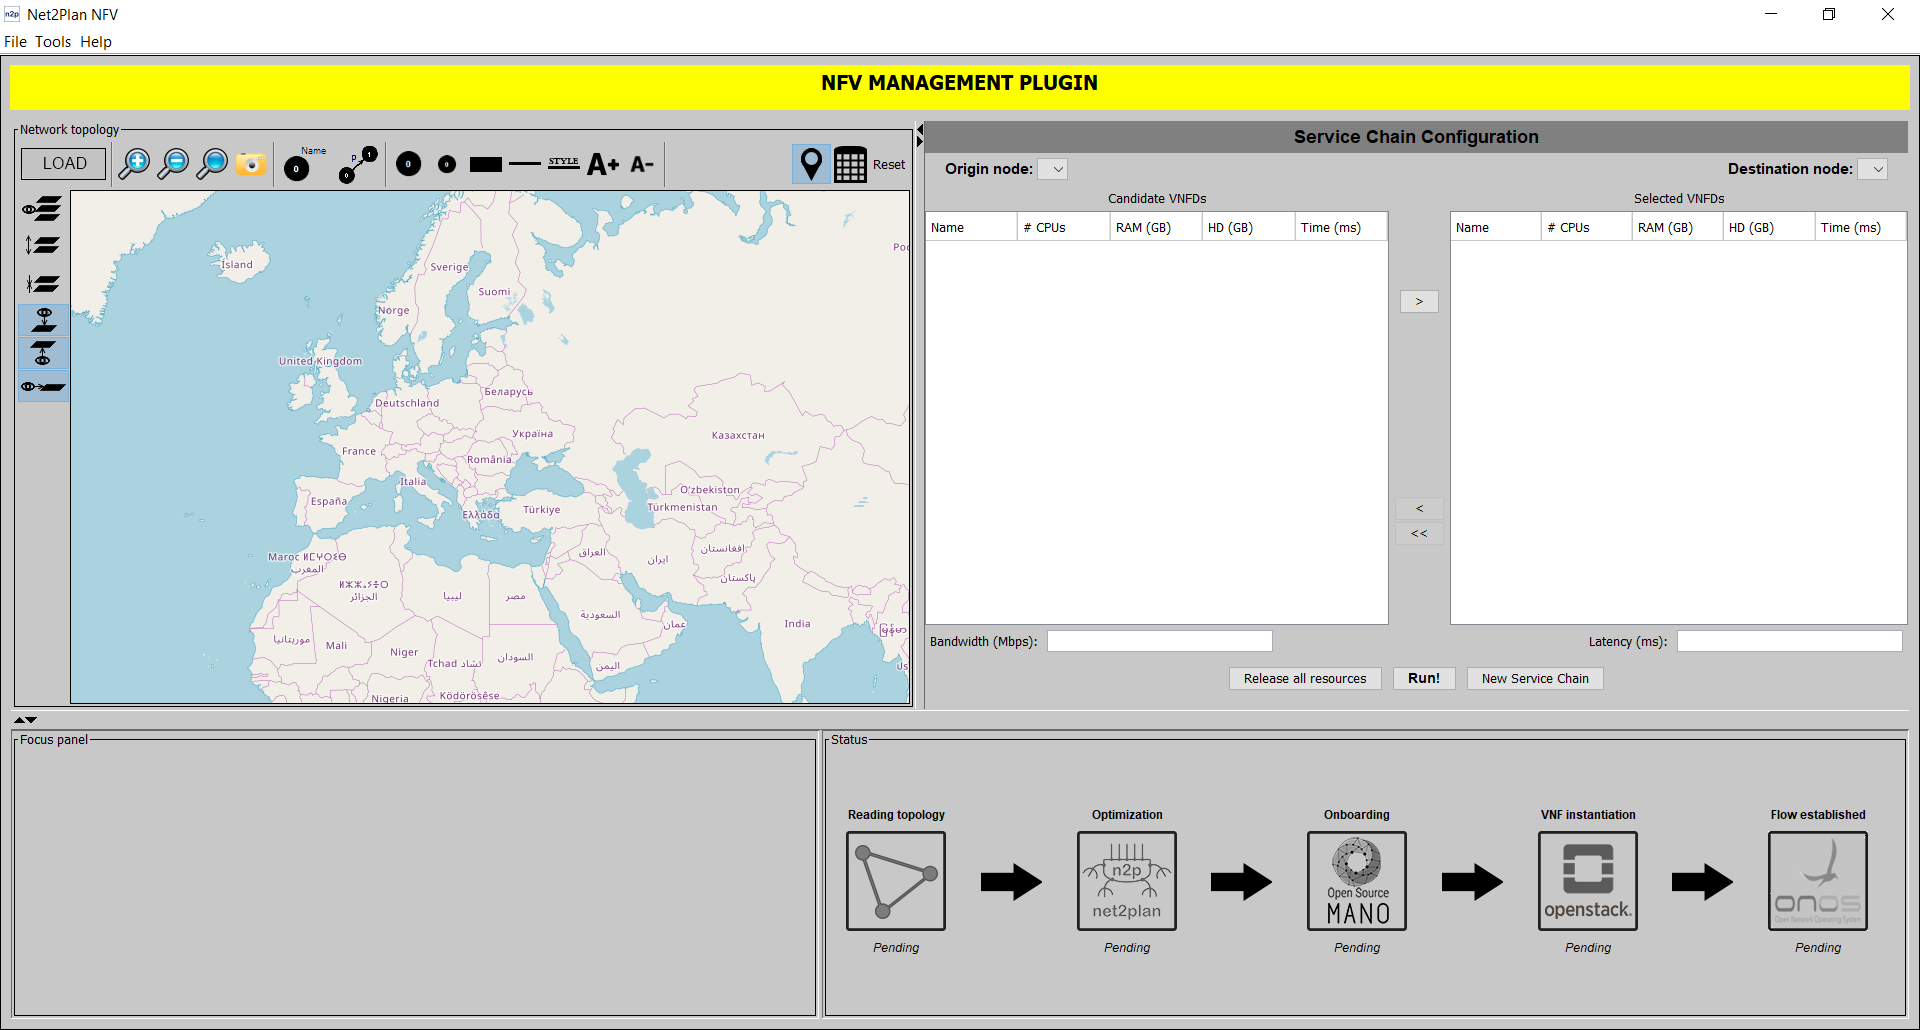
\includegraphics[width=0.9\linewidth]{imagenes/nfvplugin_dashboard}
		\caption{Interfaz gráfica del Plugin al inicio}
		\label{fig:nfvproof_inicio}
	\end{figure}
	
	\item \textbf{Paso 2.} Haciendo click en el botón LOAD, Net2Plan recibe la información referente a la red de transporte de \ac{ONOS} haciendo uso de J-ONOSClient, la información sobre los posibles \acp{VNF} a instanciar en \ac{OSM} haciendo uso de J-OSMClient y la información sobre cada \ac{VIM} de OpenStack haciendo uso de J-OpenStackClient.
	
	\item \textbf{Paso 3.} El usuario define la \textit{Service Chain} que se quiere satisfacer (nodo origen, nodo destino, secuencia ordenada de VNFs a atravesar, latencia máxima y ancho de banda) a través de la interfaz gráfica del Plugin.
	
	\clearpage
	
	\item \textbf{Paso 4.} Net2Plan recibe la información introducida por el usuario y la transfiere al \ac{LA-SCCE} para que ejecute el algoritmo que devolverá como resultado una ruta de enlaces para la \textit{Service Chain} y el \ac{VIM} donde cada \ac{VNF} debe ser instanciado.
	
		\begin{figure}[!ht]
		\centering
		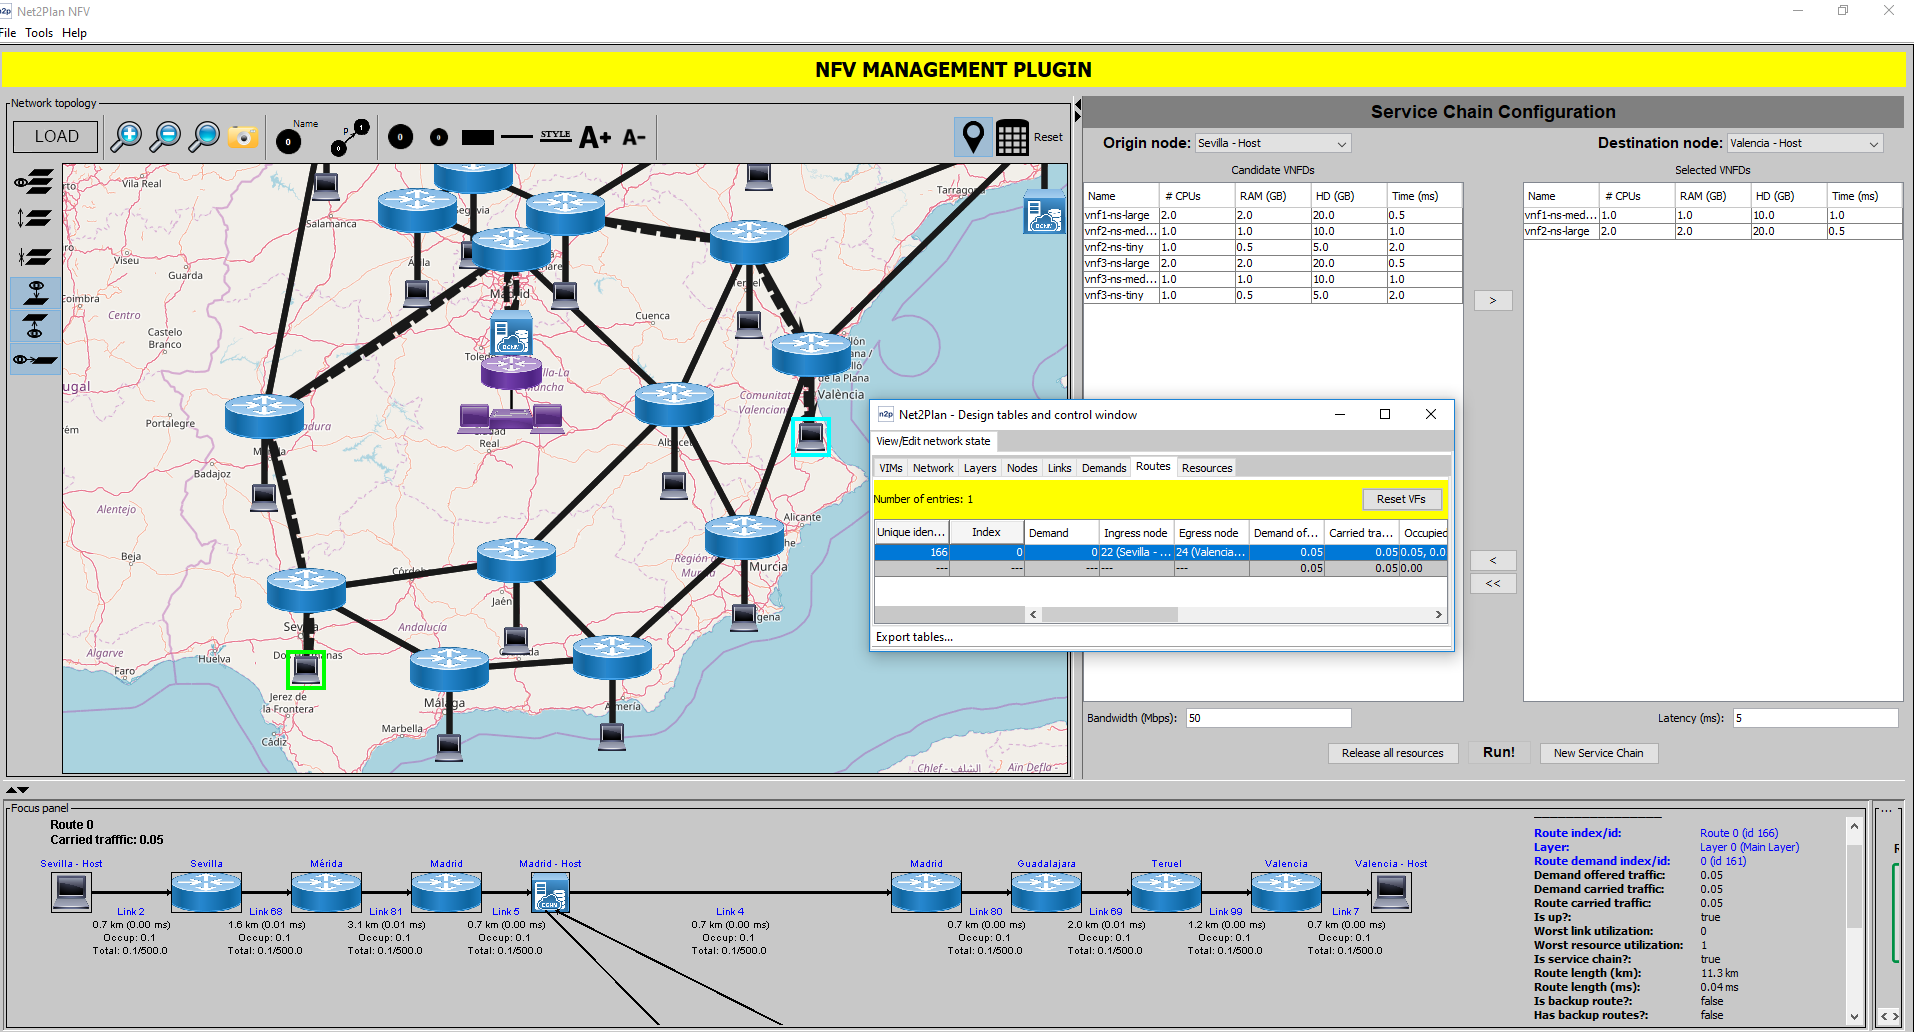
\includegraphics[width=0.9\linewidth]{imagenes/nfv_service_chain}
		\caption{Interfaz gráfica del Plugin con la ruta establecida}
		\label{fig:nfvservicechain}
	\end{figure}

	En la figura \ref{fig:nfvservicechain} se apreciar la ruta obtenida por el algoritmo en la \ac{GUI} de Net2Plan.
	
	\item \textbf{Paso 5.} Net2Plan envía la orden a \ac{OSM} haciendo uso de J-OSMClient de instanciar los distintos \acp{VNF} en los \acp{VIM} que el \ac{LA-SCCE} obtuvo como óptimos.
	
	\begin{figure}[!ht]
		\centering
		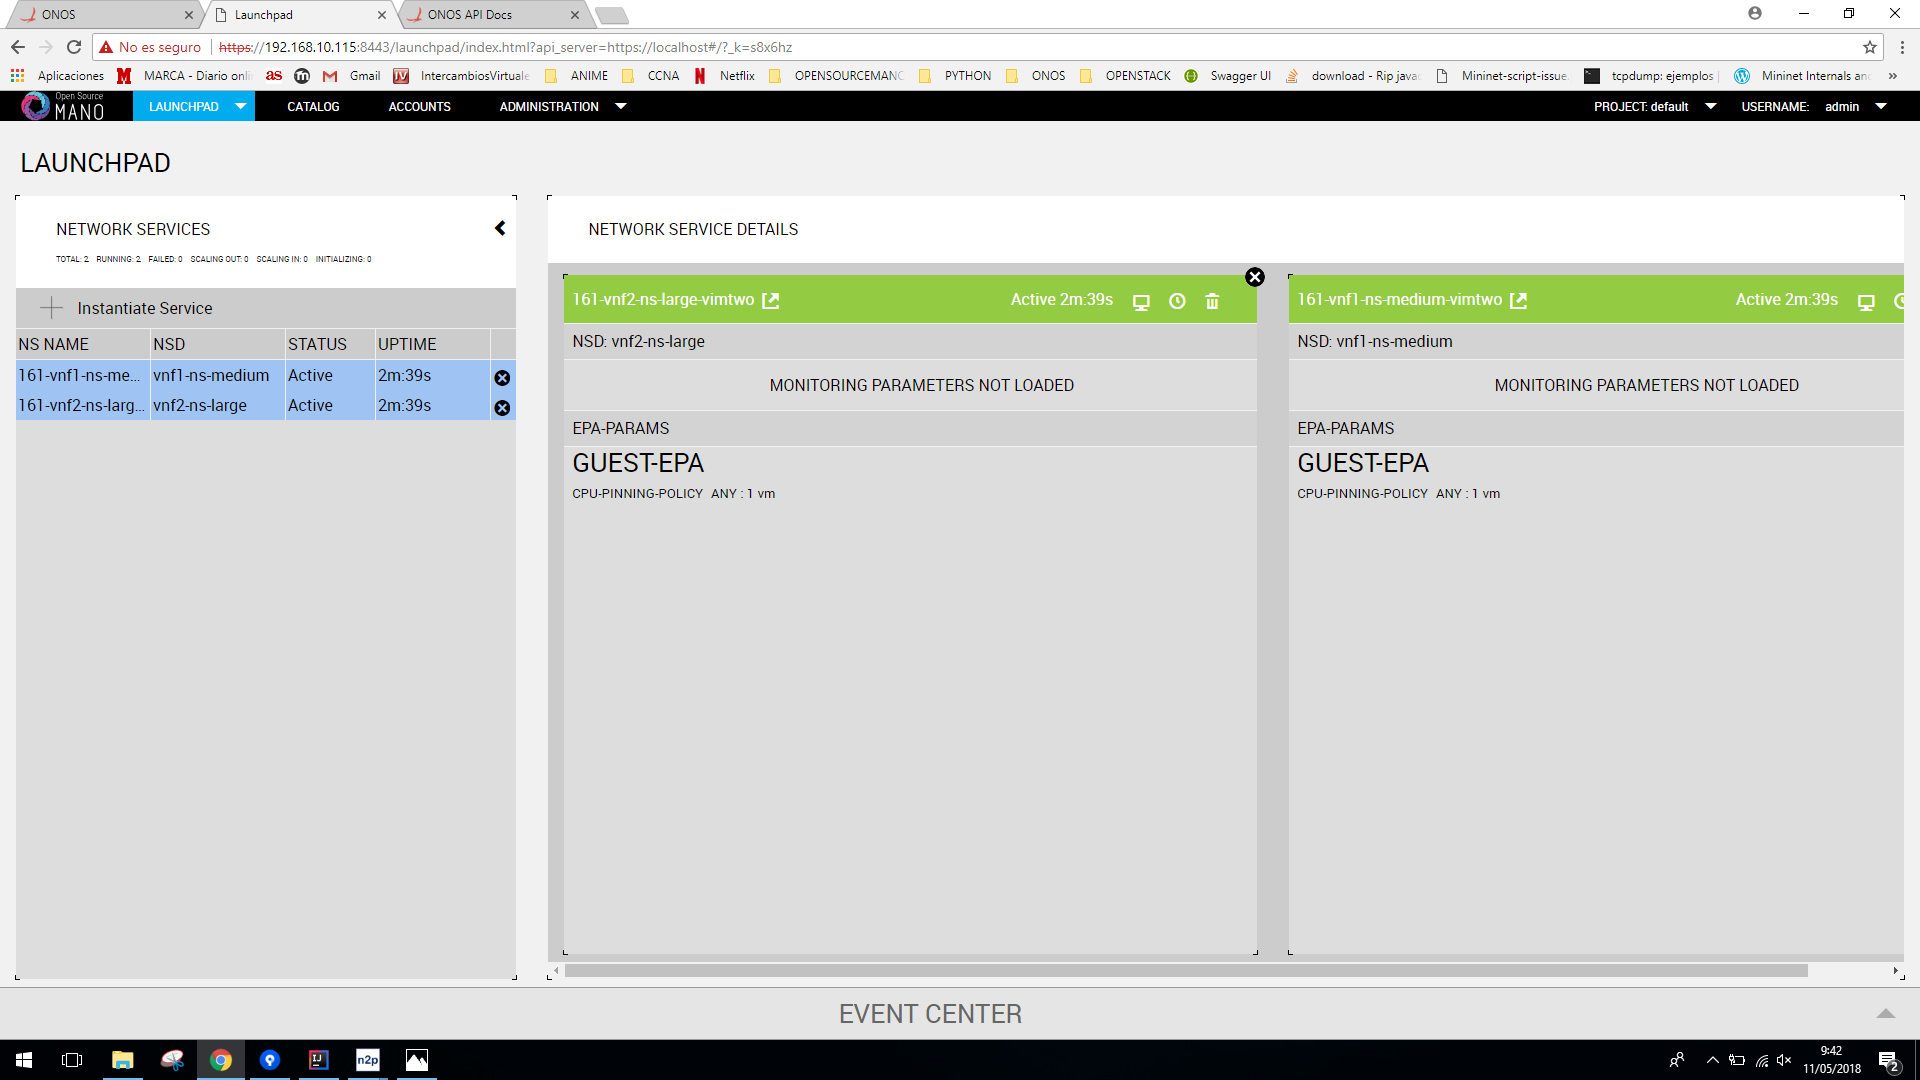
\includegraphics[width=0.9\linewidth]{imagenes/osm_vnfs}
		\caption{Interfaz gráfica de \ac{OSM} con los \acp{VNF} instanciados}
		\label{fig:osmvnfs}
	\end{figure}
	
	En la figura \ref{fig:osmvnfs} se puede apreciar como \ac{OSM} ha instanciados los \acp{VNF} en los \acp{VIM} según los cálculos del algoritmo.
	
	\item \textbf{Paso 6.} \ac{OSM} envia órdenes a los diferentes \acp{VIM} para que alojen las diferentes máquinas virtuales correspondientes a los \acp{VNF}. La comunicacion entre \ac{OSM} y OpenStack es transparente al usuario.
	
	\item \textbf{Paso 7.} Net2Plan envía la orden a \ac{ONOS}, haciendo uso de J-ONOSClient, con diferentes reglas de flujo para establecer en los diferentes \textit{switches} de la red de transporte, todo según la ruta óptima obtenida por el \ac{LA-SCCE}.
	
	\begin{figure}[!ht]
		\centering
		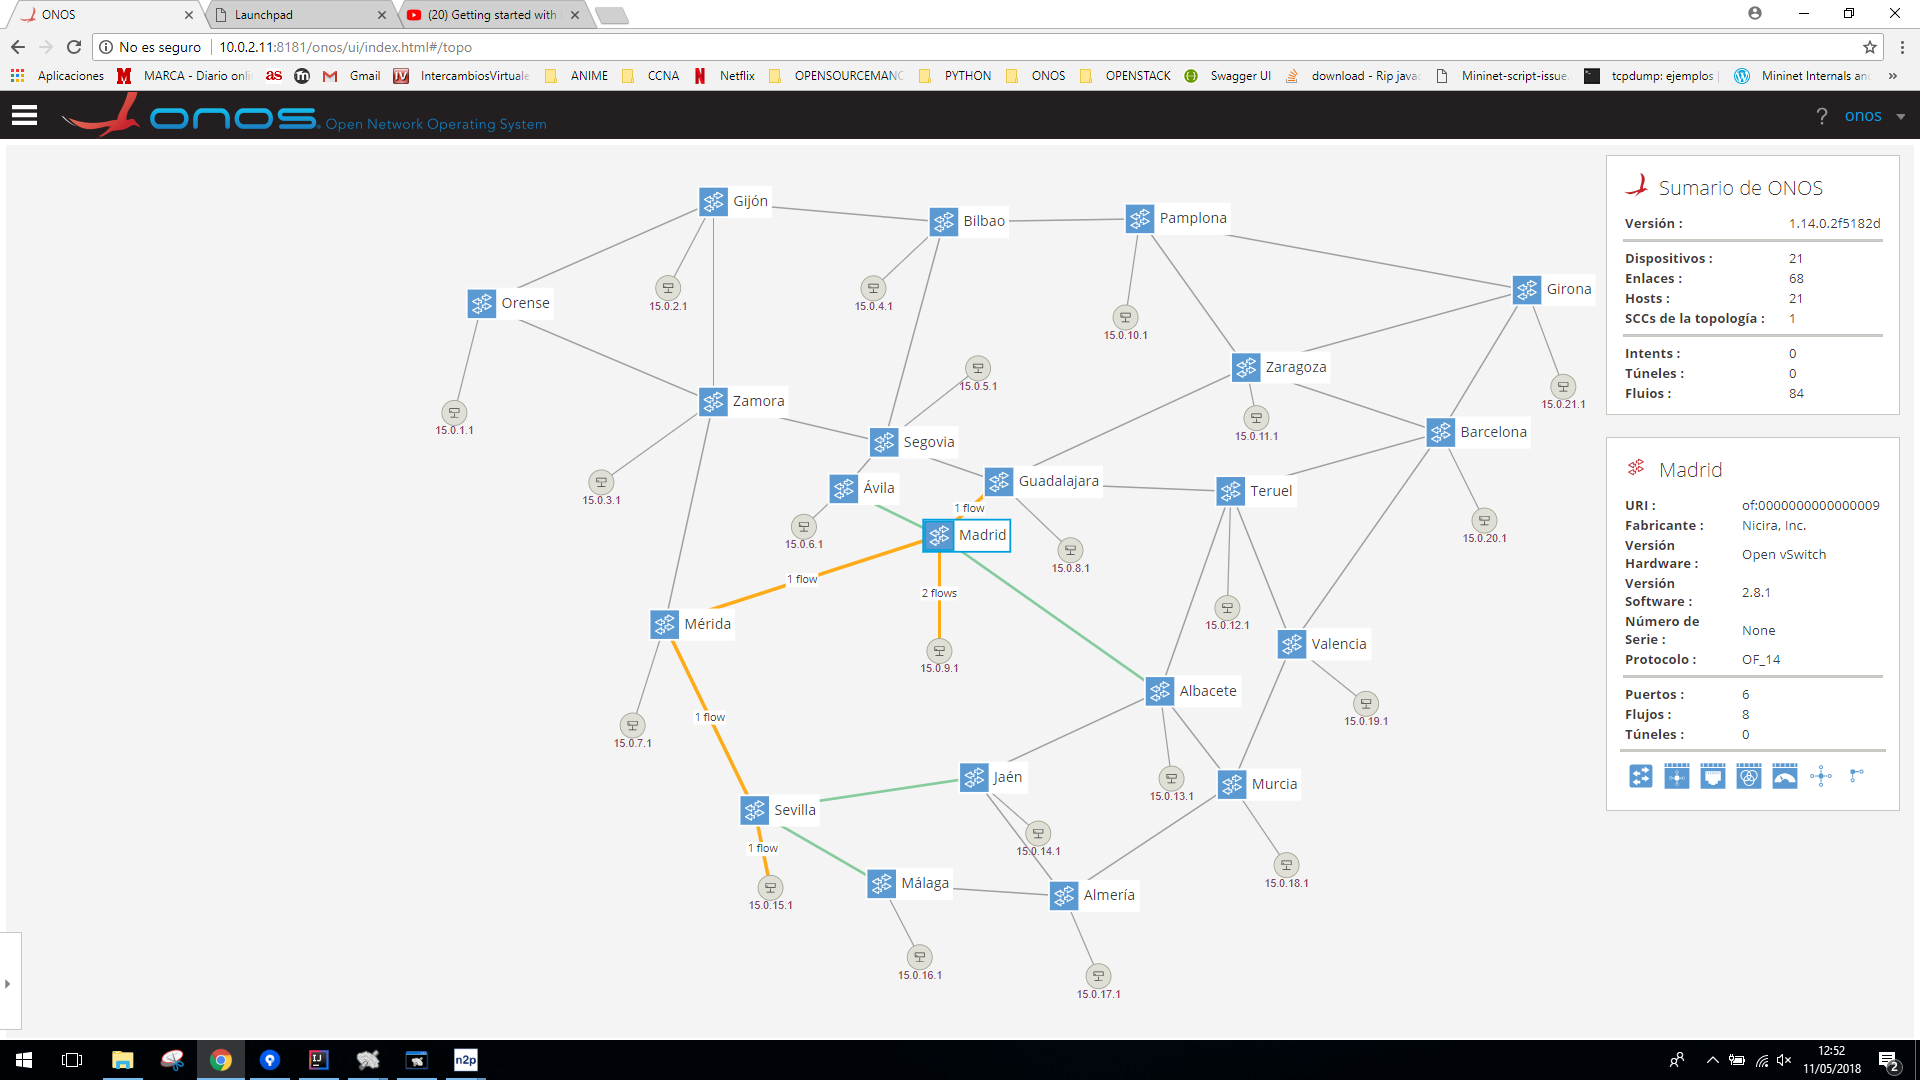
\includegraphics[width=0.9\linewidth]{imagenes/topo_onos}
		\caption{Interfaz gráfica de \ac{ONOS} con las reglas de flujo establecidas}
		\label{fig:topo_onos}
	\end{figure}

	En la figura \ref{fig:topo_onos} se puede apreciar como la ruta calculada en Net2Plan se traslada a \ac{ONOS}.

	\item \textbf{Paso 8.} Una vez establecidas las reglas de flujo en los diferentes \textit{switches} mediante OpenFlow, se realiza una prueba de conexión para asegurar que la \textit{Service Chain} está establecida y se satisface correctamente.
	
	\begin{figure}[!ht]
		\centering
		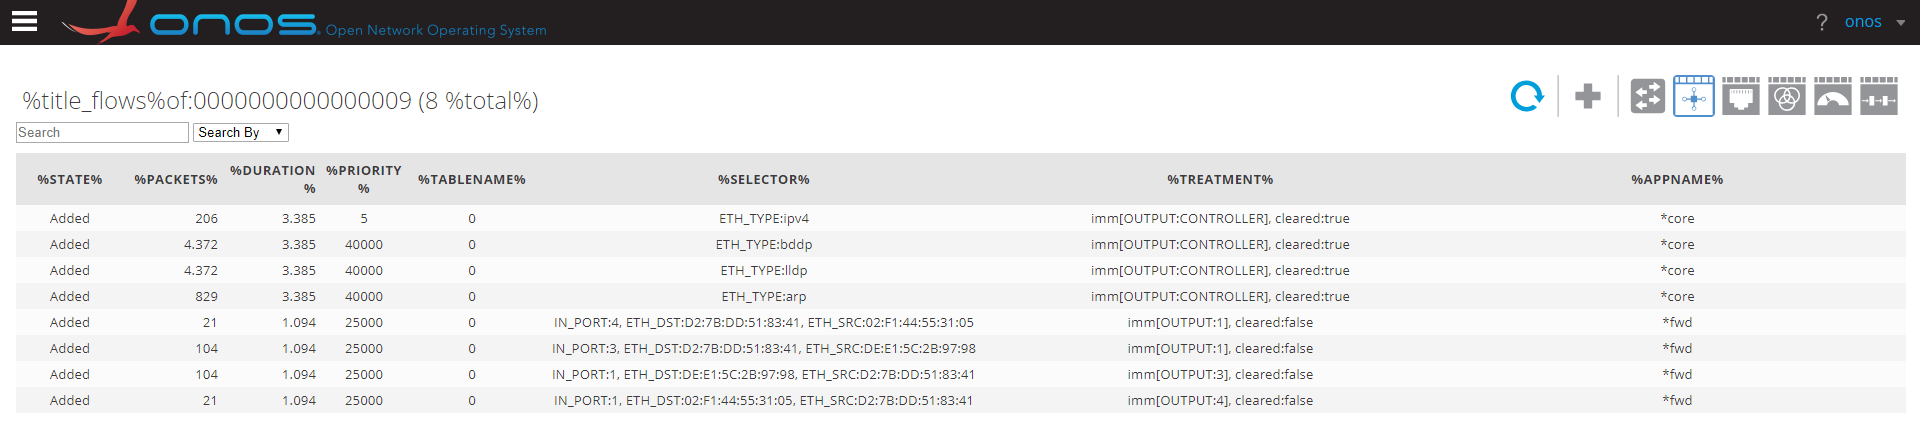
\includegraphics[width=0.9\linewidth]{imagenes/onos_flowrules}
		\caption{Prueba de conectividad en la \ac{GUI} de \ac{ONOS}}
		\label{fig:onosflowrules}
	\end{figure}

	En la figura \ref{fig:onosflowrules} se puede apreciar la instalación de reglas de flujo en \ac{ONOS} que sirven para satisfacer la \textit{Service Chain}.

\end{itemize}

Tras llevar a cabo la prueba de concepto, hay que mencionar los resultados obtenidos. Una vez instanciados los \acp{VNF} correspondientes a la \textit{Service Chain} y habiendo instalado las reglas de flujo correspondientes a la ruta óptima obtenida en los \textit{switches}, se realizan una prueba de conexión enviando un ping entre el origen y el destino. 

En la figuras \ref{fig:nfvservicechain} y \ref{fig:topo_onos} se puede observar como la ruta es la misma en ambos casos (en el plugin de Net2Plan y en \ac{ONOS}), y en la figura \ref{fig:onosflowrules} como las reglas de flujo aplicadas indican que han procesado un paquete, que corresponde al ping realizado anteriormente para validad la conectividad.

